\section{Introduction}
\label{sec:introduction}

\subsection{Climate System Components}
There are 5 main components of the climate system:
\begin{itemize}
    \item \textbf{Atmosphere}: This has the fastest response time to changes in the climate system. 
    \item \textbf{Lithosphere}: This is comprised of the crust and the upper mantle (the top layers of the Earth). It 
    interacts mainly with the atmosphere through turbulent exchanges of mass e.g. desert dust storms, volcanic eruptions.
    \item \textbf{Hydrosphere}: This is comprised of all the water on Earth. It plays a key role on the climate by means
     of providing a heat reservoir due to its large mass and heat capacity. It also affects other components of the 
     climate system through the water cycle and affects other cycles such as the carbon cycle.
    \item \textbf{Cryosphere}: This is comprised of all the ice on Earth (ice sheets, glaciers, snow fields, sea ice). 
    It is important because it reflects a lot of solar radiation back into space. It also affects the 
    \hyperlink{glo:albedo}{albedo} of the Earth (by reducing it if its cryosphere's size decreases and vice versa).
    \item \textbf{Biosphere}: This is comprised of all the living organisms on Earth. It affects the climate system by 
    means of the carbon cycle and the water cycle. This is highly sensitive to climate state.
\end{itemize}

\begin{figure}[h]
    \centering
    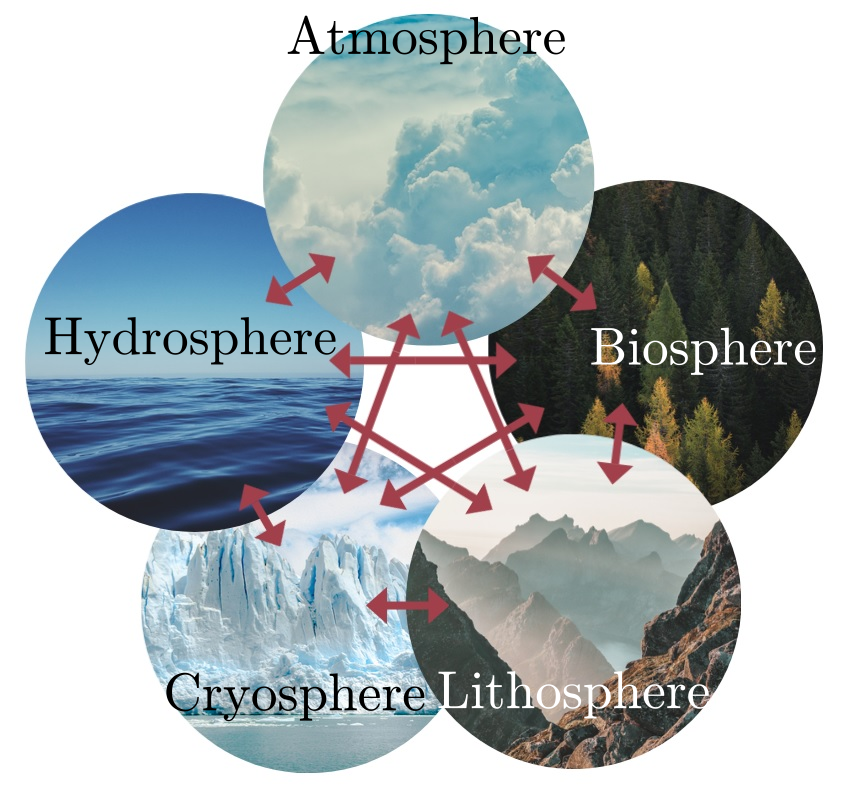
\includegraphics[scale=0.5]{figures/climate_system_components.png}
    \caption{Climate System Components}
    \label{fig:ClimateSystem}
\end{figure}

\subsection{Total Solar Irradiance}
The climate system is fundamentally driven by the sun. Energy transfer from the Sun to the Earth is only done through
EM radiation. To define this more rigorously, we assume the sun emmits \textbf{isotropically} (equally in all directions)
as a \textbf{black body}. We can reach an expression for the irradiance $I$ from the Sun reaching the \gls{TOA}:
$$
I = \sigma T_{\text{Sun}}^4 \frac{R_{\text{Sun}}^2}{R_{ES}^2} \quad \implies \quad \text{\hyperlink{glo:TSI}{TSI}} = \sigma 
T_{\text{Sun}}^4 \frac{R_{\text{Sun}}^2}{R_{ES}^2}
$$
where $\sigma$ is the Stefan-Boltzmann constant, $T_{\text{Sun}}$ is the temperature of the Sun, $R_{\text{Sun}}$ is the
radius of the Sun and $R_{ES}$ is the distance between the Earth and the Sun (radius of Earth's orbit, 1AU). A rough 
value for $I$ is $1360\ Wm^{-2}$.

Althought the \gls{TSI} is usually considered a constant, this does in fact vary on a number of timescales.
There are millenial time-scale orbital variations (Milankovitch cycles) and the Sun's own activity cycle (11 years). 
The \gls{TSI} can be measured in a number of ways, most recently by satellite measurements. The variation in 
the \gls{TSI} seen over the last few decades is of the order 1-2 $Wm^{-2}$.

\subsection{Planetary Albedo and the Earth's Emitting Temperature}
\label{sec:albedo}
At the \gls{TOA}, the only energy transfer is through EM (photon) radiation. Over time, the Earth will reach
\textbf{radiative equilibrium} where the amount of energy absorbed by the Earth is equal to the amount of energy emitted
by it at the \gls{TOA}.

\noindent Not all the energy from the Sun is absorbed by the Earth. Some of it is reflected back into space. The fraction
of energy reflected back into space is called the {\textbf{\hyperlink{glo:albedo}{planetary albedo}}}. 

The Earth, with radius $R_E$ and area $\pi R_E^2$ incident to the solar beam with \hyperlink{glo:albedo}{albedo} $\alpha_p$ 
will reach equillibrium when:
$$
4 \pi R_E^2 \sigma T_E^4 = (1 - \alpha_p) \pi R_E^2 \text{\hyperlink{glo:TSI}{TSI}} \quad \implies \quad T_E = \left(
\frac{1 - \alpha_p}{4} \right)^{\frac{1}{4}} T_{\text{Sun}} \approx 255\ K
$$

Here, we have equated the Earth's emission to the energy absorbed by it. Rearanging, we obtain the \textbf{emitting
temperature} ($T_E$) of the Earth which comes out to about $\sim 255$ K. This is much lower than the actual average surface
temperature of the Earth ($\sim 288$ K). We will see later in the course that this is because the Earth in fact has an 
atmosphere which traps heat and increases the surface temperature as to balance the energy equation.